\documentclass[12pt, toc = bibliography, english]{scrreprt} %display bibliography in table of contents
\usepackage[utf8]{inputenc} %input encoding
\usepackage[T1]{fontenc} %font encoding
\usepackage{lmodern} %font
\usepackage{babel}
\usepackage{pdfpages} %allow import of pdf
\usepackage[hidelinks]{hyperref} %do not display links underlined and in color
\usepackage{bookmark} % for hyperref
\usepackage[backend=biber, citestyle=ieee, sorting=none]{biblatex} %bibliography
\usepackage{csquotes} %german quote style
\usepackage{acro} %acronyms
\usepackage[a4paper,left=3cm, right = 2cm]{geometry} %size of document
\usepackage{setspace}
\usepackage{parskip} % do not make indentations at paragraphs
\usepackage{float} %allow [H] for images to stay where you want them
\usepackage{xcolor}
\usepackage{fancyhdr}
\usepackage{xurl} %avoid overful hbox by breaking urls everywhere
\usepackage{listings} % Für Code-Listings
\usepackage{adjustbox}
\usepackage{pgfplots}
\usepackage{tikz}
\usepackage{pgfplotstable}
% \usepackage{pgf-pie}

\definecolor{treeBlue}{HTML}{00a8f3}
\definecolor{treeGreen}{HTML}{0ed145}
\definecolor{tableGreen}{HTML}{5ea06e}
\definecolor{tableBlue}{HTML}{187eca}
\definecolor{excelOrange}{HTML}{ffcc99}
\definecolor{excelGreen}{HTML}{00b050}
% Farbdefinitionen
\definecolor{codegray}{gray}{0.90} % Hellgrauer Hintergrund
\definecolor{codeblack}{gray}{0} % Hellgrauer Hintergrund

\definecolor{codegreen}{rgb}{0,0.6,0}
\definecolor{codeblue}{rgb}{0,0,1}
\definecolor{codered}{rgb}{0.6,0,0}
\definecolor{codepurple}{rgb}{0.58,0,0.82}
\definecolor{commentcolor}{rgb}{0.5,0.5,0.5} % Kommentarfarbe

\renewcommand{\rmdefault}{lmr} % Arial
\renewcommand{\sfdefault}{lmr} % Arial
\RedeclareSectionCommand[
 beforeskip=0cm % reduce margins at chapters
]{chapter}
\fancyhead[C]{}
\fancyhead[R]{}        
\pagestyle{fancy} %fancy header: only display chapter
\fancyhead[L] {
    \leftmark{}
}                
\linespread{1.25} %entspricht 1,5 in word
% \counterwithout{figure}{chapter} %Abb.1 not Abb.[chapter].1


\lstdefinestyle{mystyle}{
   backgroundcolor=\color{codegray},  % Hintergrundfarbe
   commentstyle=\color{commentcolor},
   keywordstyle=\color{codeblue},
   numberstyle=\tiny\color{codeblack},
   stringstyle=\color{codepurple},
   basicstyle=\ttfamily\footnotesize,
   breakatwhitespace=false,
   breaklines=true,
   captionpos=b,
   keepspaces=true,
   numbers=left,
   numbersep=5pt,
   showspaces=false,
   showstringspaces=false,
   showtabs=false,
   tabsize=2,
%    language=C,
   postbreak=\mbox{\textcolor{red}{$\hookrightarrow$}\space}
}

\lstset{style=mystyle}



\DeclareAcronym{msrp}{
	short = MSRP,
	long = manufacturer's suggested retail price
}

\DeclareAcronym{csv}{
	short = CSV,
	long = Comma-separated values
}

\DeclareAcronym{vw}{
	short = VW,
	long = Volkswagen
}

\DeclareAcronym{excel}{
	short = Excel,
	long = Microsoft Excel
}

\DeclareAcronym{mpg}{
	short = MPG,
	long = miles per gallon
}

\DeclareAcronym{vscode}{
	short = VS Code,
	long = Visual Studio Code
}

\DeclareAcronym{mse}{
	short = MSE,
	long = Mean-squared error
}

\DeclareAcronym{r2}{
	short = ${r}^2$,
	long = coefficient of determination
} 
\addbibresource{sources.bib}

\begin{document}
\title{Business analytics \\ Analysis of car advertisement data}
\author{Alina Ivanova, Moritz Hangen, Simon Gosch}
\date{2024/03/24}
\maketitle

\tableofcontents
\listoffigures
\addcontentsline{toc}{chapter}{\listfigurename} %Abbildungsverzeichnis in table of content
\listoftables
\addcontentsline{toc}{chapter}{\listtablename} %Abbildungsverzeichnis in table of content

\chapter{Introduction}
As of 2023, a compound annual growth rate of 10\% was forecast for the world used car market between 2024 and 2029. There are a lot of factors that may cause such a significant growth, including shorter vehicle ownership times, changes in preferences for cars, and increasing flexibility of supply
\autocite{UsedCarMarket}.
The market growth and upward trend in the demand for cost-effective used cars 
\autocite{EuropeUsedCar} 
raise the necessity of proper price calculations for resale cars, since it affects both car dealers and clients. Prices should estimate the accurate value of the vehicle based on its condition. Moreover, the initial set price of the car is significant for the final revenue received from the dealership.
 
This paper addresses the business problem of determining competitive prices for used cars to be advertised. For the accuracy of the analysis, only one car model was chosen: the \ac{vw} Golf, as it is one of the most popular cars on the used car market in such countries as Germany, Belgium and Italy 
\autocite{misselhornDevelopmentUsedCar2024}.
The following research questions were posed: 
\newline
1) What factors influence \ac{vw} Golf's price the most? \newline
2) What is the price the \ac{vw} Golf should be advertised for? \newline
To answer the questions, correlation and linear regression is calculated. The programs used for the analysis are \ac{excel} and Orange.
The research was based on a large-scale dataset for automotive applications, which contained various data for 0.25 million used cars in the United Kingdom. For research purposes, only a part about used car advertisements was used.



\chapter{Theoretical background}
\section{Correlation}

In simple terms, a correlation coefficient shows if two variables are dependent.
The correlation coefficient varies from -1 to 1. The closer it is to extreme values, the stronger the variables are related. If the correlation coefficient is positive, that means that variables move in the same direction; for instance, when demand is growing, prices are increasing, and if demand decreases, prices go down as well. A negative correlation shows the opposite relationship. For example, when supply rises, prices drop, and vice versa. The correlation of 0 indicates that variables are independent \autocite{DaCostaLewis2005}.

\section{Linear regression}

Linear regression is a statistical tool that helps to predict the value of a targeted dependent variable based on other attributes.
An important measure in linear regression analysis is the coefficient of determination.
It represents the percentage of cases where the change in an independent variable can be explained by the change in a dependent one.
The coefficient of determination varies between 0 and 1.
The closer it is to 1, the stronger the linear relationship between variables \autocite{kumariLinearRegressionAnalysis2018}.
\section{Data}
We explored a large-scale dataset for automotive applications which originally consisted of 7 files:
\begin{itemize}
    \item "Ad\_table": Contained information about more than 0.25 million used car advertisements
    \item "Ad\_table (extra)":
    \item "Basic\_table": information about car attributes
    \item "Image\_table": car images attributes
    \item “Price\_table”: entry-level new car prices for 1998-2021
    \item “Sales\_table”: ten years car sales data in UK
    \item “Trim\_table”: trim attributes including the engine type and engine size
\end{itemize}
For our research purposes, we used “Ad\_table (extra)”.
It shows data about used car advertisements for more than 80 different car brands in 2016-2018.
The dataset contains information about cars' maker and models, month and year of the advertisement,
cars' year of registration, body type, color, ran miles, engine size in liters, and engine power in horsepower,
gearbox (automatic, annual, semi-annual), fuel type (diesel, electric, hybrid petrol/electric plug in, petrol),
the price and annual tax in pounds, wheelbase in millimeters, cars dimensions:
height, width, and length in millimeters; average miles per gallon; top speed in miles per hour; the number of seats and doors.
In addition, there were attributes for model ID and advertisement ID \autocite{huangDVMCARLargescaleAutomotive2022}.

\chapter{Analysis}
\section{Analysis method}
The goal is to make a data driven decision on how much a \ac{vw} Golf arriving at the dealership should be advertised for,
based on the car's specifications, assuming there is some kind of dependence.
To check whether this dependence exists, the correlations between the specifications and the price are evaluated.
After that, to get a model that predicts the price based on the other attributes, linear regression is used.
Its simplicity when it comes to understanding and calculating the model, as well as interpreting the results, make it well-suited
for this use case.    

\section{Data processing}
\subsection{Preprocessing in Excel}
First step of preprocessing the data is the reduction to only data points with the value \enquote{\ac{vw} Golf} for the car model attribute. Therefore, the \ac{csv} file containing the raw data is
imported into \ac{excel}, and a filter to the car model column is applied. As some cells are blank for certain attributes, another filter removing the affected rows is set for every column. 

\subsection{Preparations for Orange}
After the previous steps, the data set is still not ready to be processed in Orange. The problem is that certain cells not only contain the actual numeric value but also the 
unit. For example the column of the car's average \ac{mpg} always has the text \enquote{mpg} after the value, causing Orange to not recognize it as 
numeric value. To fix this issue, the \ac{csv} file is opened in a text editor, and its \enquote{Find and replace} functionality is used to replace the unit with blank text.
This is working as the texts,
which have to be removed, only appear in two other places, where they are manually added back. So both the \enquote{mpg} from the average \ac{mpg} column and the \enquote{L}
from the engine size column were removed like this.

\subsection{Processing in Orange}
To understand how each attribute affects the car's price, the correlations are calculated using the Pearson correlation coefficient. 
\begin{figure}[h]
    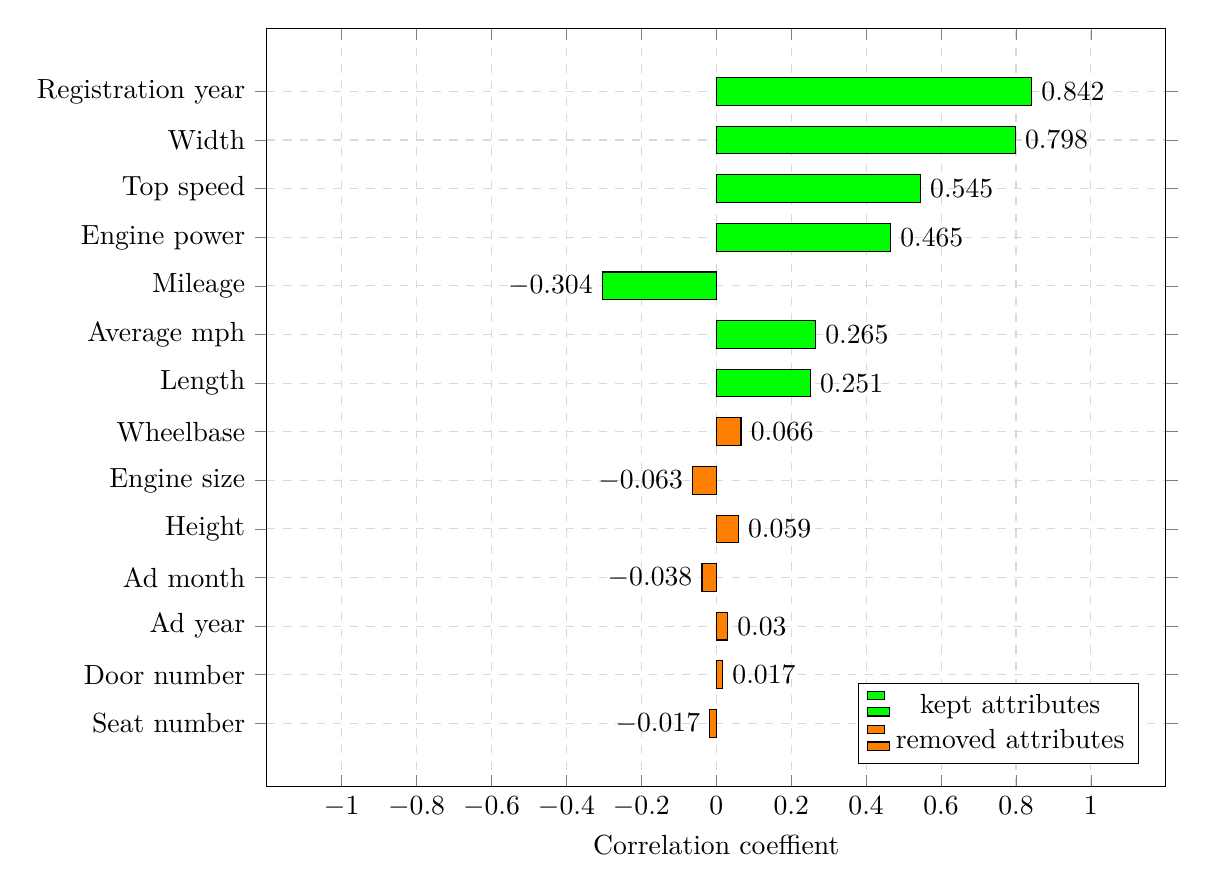
\begin{tikzpicture}
        \begin{axis}[
            xbar,
            xmin=-1.2,
            xmax=1.2,
            xtick={-1,-0.8,-0.6, -0.4, -0.2, 0, 0.2, 0.4, 0.6, 0.8, 1},
            legend pos=south east,
            grid=major, grid style={dashed,gray!30},
            width=13cm,
            xlabel={Correlation coeffient},
            symbolic y coords={Seat number,Door number,Ad year,Ad month,Height,Engine size,Wheelbase,Length,Average mph,Mileage,Engine power,Top speed,Width,Registration year},
            ytick={Seat number,Door number,Ad year,Ad month,Height,Engine size,Wheelbase,Length,Average mph,Mileage,Engine power,Top speed,Width,Registration year},
            nodes near coords,
            nodes near coords align={horizontal},
            every node near coord/.style={/pgf/number format/fixed, /pgf/number format/precision=3},
            /pgf/bar shift={0pt},
            ]
            \addplot [fill=green] coordinates {
                (0.251,Length)
                (0.265,Average mph)
                (-0.304,Mileage)
                (0.465,Engine power)
                (0.545,Top speed)
                (0.798,Width)
                (0.842,Registration year)
                };
            \addplot [fill=orange] coordinates {
                (-0.017,Seat number)
                (0.017,Door number)
                (0.03,Ad year)
                (-0.038,Ad month)
                (0.059,Height)
                (-0.063,Engine size)
                (0.066,Wheelbase)
                };
            \legend{kept attributes, removed attributes}
        \end{axis}
    \end{tikzpicture}
    \caption{Correlation with the price attribute}
    \label{fig:correlationdiagram}
\end{figure}
\par
\autoref{fig:correlationdiagram} shows a horizontal bar chart visualizing the correlation coefficient for each attribute.
As a bar chart lists the different values of the coefficients side by side in an easy-to-read way, it is perfect for the 
given purpose of focusing on comparison between the attributes. 
The horizontal layout allows good readability for the long labels and is more suitable for placing the actual values next to the
bars, as there are no space limitations along the y-axis. 
\par
Having the results of the correlation analysis allows to answer the first research question: \enquote{What factors influence Volkswagen Golf's price the most?}.
\autoref{fig:correlationdiagram} provides the answer, as the attributes are listed from highest to lowest influence on the price. Those highlighted in green
have a significant impact, while the rest do not. Therefore, those highlighted in orange are not taken into account for the further data analysis.

\par
In the next step, not only the attributes with low correlation but also the non-numeric ones are removed. This is the case as they can't be used in the calculation
of the linear regression model without further preprocessing. These additional preprocessing steps are not performed as the resulting linear regression
model is already very good. 
Additionally, the price is set as target value for the linear regression calculation.

\par
As a final step, the data set is split into training and test data, and the linear regression model is calculated based on the
training data. Insights about the training split, as well as quality and specifications of the model, are discussed in the next section of the report. 

\section{Linear regression model}
\subsection{Specifications}
For the calculation of the linear regression model, a training split of 60\% training and 40\% test data is used.
When testing the model, the results are very satisfactory with a \ac{mse} of 3750250.922 and \ac{r2} of 0.912.
Especially, the \ac{r2} being very close to 1 indicates a high linear relationship between the model and the target attribute,
which means that the model predicts the price accurately.

\subsection{Visualization}
The reason for visualizing the linear regression model is that it is always easier to analyze and interpret visual 
results rather than only working with numeric values.
Used for that matter is a scatter plot, shown in \autoref{fig:linearregressiondiagram}. 
\begin{figure}[h]
    \begin{tikzpicture}
        \begin{axis}[
            clip mode=individual,
            legend pos=south east,
            xmin=400,
            xmax=20000,
            ymin=400,
            ymax=20000,
            xlabel={Actual price \lbrack\pounds\rbrack},
            ylabel={Model's calculated price \lbrack\pounds\rbrack},
            xtick={2000, 6000, 10000, 14000, 18000},
            ytick={2000, 6000, 10000, 14000, 18000},
            width=13cm,
            scaled ticks=false,
            tick label style={/pgf/number format/fixed},
            y label style={yshift=1.2em}
            ]
        \addplot [mark=none,color=blue,style=very thick]
          table [y={create col/linear regression={y=model_price}}, col sep=comma] {./other/Linear_regression.csv};
          \addlegendentry{Regression line}  
          \addplot [mark=*,color=red,only marks, fill opacity = 0.35, draw opacity = 0]
          table [x=actual_price, y=model_price, col sep=comma] {./other/Linear_regression.csv};
                 
        \end{axis}
      \end{tikzpicture}
    \caption{Plotted Linear Regression Model}
    \label{fig:linearregressiondiagram}
\end{figure}
\par
Scatter plots are optimal to show the relationship between two variables, in this case, the actual price from the test data 
and the price predicted by the linear regression model. The closer the data points are to the regression line, the 
better the model performs. By knowing this, it is easy to analyze the quality of the model, even without any prior knowledge.
So, when looking at \autoref{fig:linearregressiondiagram}, one can see that the data points portray the regression line 
quite precisely. This reinforces the prior statement that the linear regression model is very good.


\chapter{Results}
\section{Model usage}\label{model_usage_section}
After examining the theoretical background of the regression model, it can be applied to example data to investigate its behavior.
\subsection{Assessing expectations}
Intuitively, the vehicle's mileage should have an inverse relationship to the predicted advertisement price.
To evaluate if the model also follows this behavior, it was applied to manually created data differentiating only by mileage.
\begin{table}[H]
    \begin{adjustbox}{width={\textwidth}}
        \begin{tabular}{|c|c|c|c|c|c|c|c|}
            \hline
            Registration & \textbf{Mileage} & Horse- & Width & Length & Average & Top speed & \textbf{Predicted price} \\[-1ex]
            year         & \textbf{(mi)}    & power  & (mm)  & (mm)   & mpg     & (mph)     & \textbf{(£)}             \\ \hline
            2017         & \textbf{60000}   & 135    & 2027  & 4284   & 49      & 116       & \textbf{16157}           \\\hline
            2017         & \textbf{130000}  & 135    & 2027  & 4284   & 49      & 116       & \textbf{13828}           \\\hline
        \end{tabular}
    \end{adjustbox}
    \caption{Impact of mileage on recently registered cars}
    \label{mileage_data_new_car}
\end{table}
As evident in \autoref{mileage_data_new_car}, a higher mileage in fact reduces the predicted price.
However, for an over 2-fold increase in miles, the depreciation is with 14.4 \% not as high as initially expected.
\par
While comparing two otherwise identical cars, it should be noted that the other values still measurably contribute to the
result.
\newline
In particular the registration year, which, as shown before, strongly correlates with the target variable, has an effect on the limited
influence of the mileage here.
Given the data set's sampling of data up to 2018, both of the \ac{vw} Golfs in \autoref{mileage_data_new_car} have been first registered very recently,
thus the base price is higher.
If the same example is applied to cars registered in 2010, the influence of the mileage grows.
\begin{table}[H]
    \begin{adjustbox}{width={\textwidth}}
        \begin{tabular}{|c|c|c|c|c|c|c|c|}
            \hline
            \textbf{Registration} & \textbf{Mileage} & Horse- & Width & Length & Average & Top speed & \textbf{Predicted price} \\[-1ex]
            \textbf{year}         & \textbf{(mi)}    & power  & (mm)  & (mm)   & mpg     & (mph)     & \textbf{(£)}             \\ \hline
            \textbf{2010}         & \textbf{60000}   & 135    & 2027  & 4284   & 49      & 116       & \textbf{11122}           \\\hline
            \textbf{2010}         & \textbf{130000}  & 135    & 2027  & 4284   & 49      & 116       & \textbf{8793}            \\\hline
        \end{tabular}
    \end{adjustbox}
    \caption{Influence of mileage on older cars}
    \label{mileage_data_old_car}
\end{table}
As shown in \autoref{mileage_data_old_car}, the gap between the two otherwise identical vehicles has widened to 20.9 \%, an increase by 45.3 \%.
Potential reasons for the strong correlation between year and target value will be investigated further in \autoref{year_to_price_correlation}.
Nevertheless, for that small subset of data, the efficacy of the model is evident.
\subsection{Usage of example data}
However, this small example is not cohesive enough to demonstrate the ability to solve the overall business problem.
To apply the model to a day-to-day use case as it regularly appears in a dealership,
it was used to predict the advertisement price of four automobiles.
\begin{table}[H]
    \begin{adjustbox}{width={\textwidth}}
        \begin{tabular}{|c|c|c|c|c|c|c|c|}
            \hline
            Registration & Mileage & Horse- & Width & Length & Average & Top speed & \textbf{Predicted price} \\[-1ex]
            year         & (mi)    & power  & (mm)  & (mm)   & mpg     & (mph)     & \textbf{(£)}             \\ \hline
            2014         & 180000  & 110    & 1799  & 4204   & 45      & 110       & \textbf{5601}            \\\hline
            2016         & 150000  & 120    & 2027  & 4255   & 48      & 112       & \textbf{12130}           \\\hline
            2018         & 80000   & 130    & 2027  & 4255   & 50      & 115       & \textbf{16136}           \\\hline
            2015         & 190000  & 115    & 1799  & 4204   & 44      & 108       & \textbf{5819}            \\ \hline
        \end{tabular}
    \end{adjustbox}
    \caption{Model application to four business use cases}
    \label{predicted_price_realworld_data}
\end{table}
\autoref{predicted_price_realworld_data} illustrates that the model is able to set a competitive advertisement price
for a \ac{vw} Golf. As its performance with \ac{r2} = 0.912 is very good, it can be seen as a reliable source of information for the dealer.
Thus, he does not have to rely solely on human estimate but can instead decide based on a data driven prediction, solving research question two therewith. 
\section{Findings}
In \autoref{model_usage_section} the application of the model to exemplary vehicles has been demonstrated.
Here, some trends that could have already been anticipated after the correlation analysis, have emerged more clearly.
\subsection{Correlation: Horsepower, Price}
\label{subsectionhpprice}
Among the essential specifications of a vehicle is its power, measured in horsepower, significantly influencing price with a correlation coefficient of 0.465.
It affects the maximum acceleration, the top speed, the fuel consumption and other key indicators of a car's capabilities.
The improved performance is a reason why customers are willing to spend extra for a more powerful Golf.
\subsection{Correlation: Mileage, Price}
Mileage as a parameter can be seen as an indicator for wear of the vehicle.
Apart from that, maintenance parts are closer to their end of life and need to be replaced sooner,
which costs customers money and time.
\par
Looking at the data in a scatter-plot in \autoref{mileagepricediagram}, it can be seen that there is a steep decline of the vehicle's value in the beginning up to about 50000 miles,
with the effect of mileage on the price notably decreasing from roughly 100000 mi onwards.
\begin{figure}[H]
    \begin{tikzpicture}
        \begin{axis}[
                clip mode=individual,
                legend pos=south east,
                xmin=0,
                xmax=200000,
                ymin=0,
                ymax=25000,
                xlabel={Mileage \lbrack mi\rbrack},
                ylabel={Price \lbrack\pounds\rbrack},
                xtick={0, 40000, 80000, 120000, 160000},
                ytick={0, 5000, 10000, 15000, 20000},
                width=13cm,
                scaled ticks=false,
                tick label style={/pgf/number format/fixed},
                y label style={yshift=1.2em}
            ]
            \addplot [mark=*, only marks, color = red, fill opacity = 0.35, draw opacity = 0, mark size = 3pt]
            table [x=Runned_Miles, y=Price, col sep=comma] {./other/runned_miles.csv};
        \end{axis}
    \end{tikzpicture}
    \caption{Effect of mileage on price}
    \label{mileagepricediagram}
\end{figure}

A potential reason for this could be that once vehicles reach certain thresholds, most of the common maintenance has already been executed, so
a high distance travelled becomes an indicator of the car's reliability, countering the diminishing effect on the price to a certain extent.
\par
This also means that the relationship between the two markers, resembling the arm of a parabola and therefore a polynomial function,
gives the linear Pearson correlation only limited meaningfulness.
Nevertheless, its negative coefficient of -0.304 is in line with predictions, albeit not as strong.

\subsection{Correlation: Engine size, Price}
The engine displacement, informally also referred to as engine size, describes the volume of air and fuel inside an engine's pistons \autocite{EngineDisplacement2024}.
By definition, it is also directly related to its power output, in particular in older vehicles.
\par
Given that, the intuitive prediction is that it will positively correlate with the final price.
However, the analysis has shown it is not significant, with the coefficient of -0.063 approaching 0.
\par
Exploring the correlation of the engine size with other parameters, the lack of effect on the final price can be explained by looking at
three key indicators:
\begin{itemize}
    \item \textbf{Top speed: }
          With 0.552, there is a significant effect of the engine size on the top speed, which in turn increases the predicted value of the Golf.
    \item \textbf{Registration year: }
          There is a measurable trend that for newer cars, the engines become smaller, notable by a coefficient of -0.295.
          Due to the strong effect of the registration year on the predicted price, the higher engine sizes negatively influence the target value,
          compensating the aforementioned effect of top speed.
    \item \textbf{Horsepower: }
          In newer cars, horsepower is not as limited by engine size as in the past \autocite{WhatEngineDisplacement}.
          Looking at the correlation value of -0.076, this effect is also resembled in VW Golfs. Thus, as shown in \autoref{subsectionhpprice}, one of the deciding factors determining the end price 
          is not related to the engine size for \ac{vw} Golf.
\end{itemize}
To conclude, the two measurable effects even each other out and for the horsepower, where correlation might be present, there is not any, unexpectedly rendering the
engine size negligible for the analysis.

\subsection{Correlation: Width, Price}
At the first glance, a very strong tie between the width of a Golf and its advertisement price is not clear.
From a potential customer's perspective, the width of a car can be a deciding factor, for example when it comes to
narrow parking spots and small neighborhood roads.
Nonetheless, there is a strong positive correlation with the target value, implying that the dimensions of the car
could play a deciding factor in the purchase process.
\par
Investigating the matter based on the data, the reason for the connection between width and price becomes evident:
The width is very positively correlated with the registration year, which in turn is very strongly correlated with the Golf's advertisement price.
This can be attributed to the fact that VW Golfs get wider every model generation, as for instance a VW Golf V is 1759 mm,
while the current 8th generation's width is already 1789 mm \autocite{VolkswagenGolfTechnical}.
\par
Overall, there is a clear trend observable that in line with the registration year, the width increases,
resulting in the unforeseen correlation of 0.715.

\subsection{Correlation: Year, Price} \label{year_to_price_correlation}
As expected, there is a relationship in between the registration year of the car and the final price.
However, its strength with 0.842 is unprecedented and can not solely be clarified by the analyzed data.
The main reason for this is the absence of the exact model generation (Golf V, Golf VI, Golf VII...), as well as its respective \ac{msrp}, in the data.
Nonetheless, it can be assumed that year of registration is approximately equal to the manufacturing date and therefore also to the model.
\par
As prices have risen between the model generations, for instance a 16.3 \% price increase happened between comparable models of Golf V and Golf VII \autocite{DuelVWGolf},
it can be expected that this trend is reflected in advertisement prices as well.
Additionally, newer cars include more optional features which can drive up the price if they are present.
If this affects the price in the given case cannot be checked using the available data,
as there is no notice of a car's selected options.
\par
To add to that, there might also be differences in a car's maintenance cost and reliability depending on the exact model, manifesting in price differences in pre-owned vehicles.
Newer models can also contain more innovations, whose absence can make older vehicles  disproportionately less attractive, with features such as air conditioning, heated seats,
navigation and more being considered standard nowadays.
\par
Overall, trends and innovations that originate from the cost and behavior of new vehicles also manifest in the data set.
By indirectly specifying the model, the registration year is thus a strong indicator of a Golf's future advertisement price.

\chapter{Conclusion}
\section{Limitations of the analysis}
\subsection{Recency of the data}
The training data has been collected between 2016 and 2018, thus even the most recent data
is now over 5 years old. Given recent events such as the steep increase of inflation
and the COVID-19 pandemic, predictions by the model might not accurately reflect current trends.

\subsection{Lack of sales data regarding advertisement}
Additionally, while the given dataset includes conclusive data regarding the advertisement price of cars in the used vehicle market,
there is no indicator given, whether the car was actually sold at the price that it has been advertised for. 
\newline
Nevertheless, while one may anticipate a few dealerships to over or underestimate their prices,
considering the scale of the dataset, that effect levels out for the overall market.
However, evaluating whether there is a trend that pre-owned cars are systematically under- / overpriced in commercials
is only possible if you compare the given data set to real sales information.

\section{Further research topics}
Given the scale of the available data, more potential research questions may also be examined. 

\subsection{Inter-model comparison of findings}
The analysis is currently only valid for the small subset of the data including the \ac{vw} Golf. 
To elevate generalizability to the whole used vehicle market and to assess potential disparities as well as similarities among
car models, expanding the scope to the entirety of available data is recommended.  
\subsection{Assess value depreciation}
After evaluating inter-model differences, a possible further research topic is the comparison of each car's new price
to its future advertisement prices. For each model in the advertisement dataset, there is a corresponding data point
in the "basic information" table that contains, among others, the \ac{msrp}. 
\newline
With that information, the following questions could be analyzed: 
\begin{itemize}
\item Which model retains the most value compared to its \ac{msrp}?
\item Given five years of use, which car's price decreased the most?
\item Is there a correlation between value depreciation and the manufacturer of the car?
\end{itemize}
This information can be useful for customers considering the purchase of a new car in order to assess its potential resale value in the future.

\section{Résumé}

The conducted analysis provides a data-driven approach to the business problem of a competitive advertisement price of a given \ac{vw} Golf.
After preparing the raw data, key influences have been separated using Pearson-correlation and used to train a linear regression model.
\par
Considering the parameters 
\begin{itemize}
    \item Registration year
    \item Mileage (mi)
    \item Horsepower
    \item Width (mm)
    \item Length (mm)
    \item Average mpg
    \item Top speed (mph)
\end{itemize}
it accurately predicts a suitable advertisement price with $R^2 = 0.927$, solving the business problem thereby.
The end results mostly align with logical assumptions, for instance that newer cars sell for higher prices, yet also reveal
surprising behaviors such as the significant effect of the Golf's width.
To summarize, they provide further insight by revealing each factor's contribution to the vehicle's advertisement price and investigating their cause.
\par
Given those results, further potential research areas are examined and left open for future analysis. 
%TODO: move up before further research and limitations 
%TODO: Answer research questions



\printbibliography
\end{document}
